%iffalse
\let\negmedspace\undefined
\let\negthickspace\undefined
\documentclass[journal,12pt,onecolumn]{IEEEtran}
\usepackage{cite}
\usepackage{amsmath,amssymb,amsfonts,amsthm}
\usepackage{algorithmic}
\usepackage{graphicx}
\usepackage{textcomp}
\usepackage{xcolor}
\usepackage{txfonts}
\usepackage{listings}
\usepackage{enumitem}
\usepackage{mathtools}
\usepackage{gensymb}
\usepackage{comment}
\usepackage[breaklinks=true]{hyperref}
\usepackage{tkz-euclide} 
\usepackage{listings}
\usepackage{gvv}                                        
%\def\inputGnumericTable{}                                 
\usepackage[latin1]{inputenc}                                
\usepackage{color}                                            
\usepackage{array}                                            
\usepackage{longtable}                                       
\usepackage{calc}                                             
\usepackage{multirow}                                         
\usepackage{hhline}                                           
\usepackage{ifthen}                                           
\usepackage{lscape}
\usepackage{tabularx}
\usepackage{array}
\usepackage{float}


\newtheorem{theorem}{Theorem}[section]
\newtheorem{problem}{Problem}
\newtheorem{proposition}{Proposition}[section]
\newtheorem{lemma}{Lemma}[section]
\newtheorem{corollary}[theorem]{Corollary}
\newtheorem{example}{Example}[section]
\newtheorem{definition}[problem]{Definition}
\newcommand{\BEQA}{\begin{eqnarray}}
\newcommand{\EEQA}{\end{eqnarray}}
\newcommand{\define}{\stackrel{\triangle}{=}}
\theoremstyle{remark}
\newtheorem{rem}{Remark}

% Marks the beginning of the document
\begin{document}
\bibliographystyle{IEEEtran}
\vspace{3cm}

\title{1-1.5-12}
\author{AI24BTECH11011 - Himani Gourishetty}
\maketitle
\bigskip


\renewcommand{\thefigure}{\theenumi}
\renewcommand{\thetable}{\theenumi}
\begin{enumerate}
    \item In what ratio does the point $\vec{P}\brak{-4,y}$ divide the line segment joining the points $\vec{A}\brak{-6,10}$ and $\vec{B}\brak{3,-8}$? Hence, find the value of y.\\
    \textbf{Solution:}
    Given,\\
\begin{table}[h!]    
\centering
\begin{tabular}[12pt]{ |c|c|c|}
\hline
\textbf{Variable} & \textbf{Description} & \textbf{formula}\\ 
\hline
$\vec{A}\brak{x1,y1}$ & $\brak{k+1,2k}$  & - \\
\hline 
$\vec{B}\brak{x2,y2}$ & $\brak{3k,2k+3}$ & - \\
\hline
$\vec{C}\brak{x3,y3}$ & $\brak{5k-1,5k}$ & - \\
\hline 
Area & Area formed by the 3 points & $x1\brak{y2-y3}+x2\brak{y3-y1}+x3\brak{y1-y2}\\
\hline
\end{tabular}

\label{q2}
\end{table}
   \\ By section formula,
 \begin{align}
\vec{P}=\brak{\frac{\vec{A}+n\vec{B}}{1+n}}\\
\myvec{-4 \\ y} =\frac{\myvec{-6 \\ 10}+n\myvec{3 \\ -8}}{1+n}\\
 \myvec{-4\brak{2+n} \\ y\brak{1+n}}=\myvec{-6+3n \\ 10-8n}\\
\end{align}
on comparing,
 \begin{align}
n=\frac{2}{7}\\
y=\frac{10-8\brak{\frac{2}{7}}}{1+\frac{2}{7}}\\
 y=6
  \end{align}
point $\vec{P}$ divides the line segment $AB$ in the ratio 2:7.
    
\end{enumerate}
\begin{figure}[h!]
   \centering
   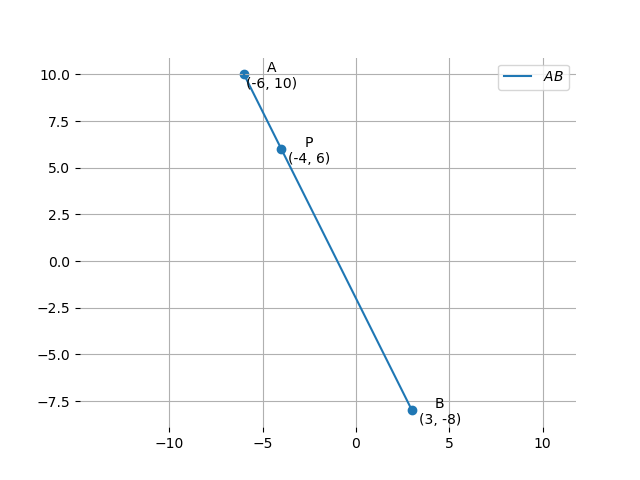
\includegraphics[width=0.7\linewidth]{figs/plot2.png}
   \label{q2}
\end{figure}


\end{document}
